\documentclass[dvipdfmx,12pt]{beamer}
\usepackage{bxdpx-beamer}
\usepackage{pxjahyper}
\usepackage{tikz}
\usepackage{here}
\usepackage{graphicx}
\renewcommand{\kanjifamilydefault}{\gtdefault}

\usepackage{amsmath}
\usepackage{amsfonts}
\usepackage{amssymb}
\usepackage{color}
\usepackage{tcolorbox}
\usepackage{forest}

\usetikzlibrary{arrows.meta}
\usetikzlibrary{positioning}

\usetheme{metropolis}  

% blockのスタイルをカスタマイズ
\setbeamercolor{block title}{bg=blue!30,fg=black} % タイトルの背景色とテキストの色
\setbeamercolor{block body}{bg=blue!10,fg=black} % ボディの背景色とテキストの色

\usepackage[usetype1]{uline--}

\title{第1回MPC勉強会}
\author{鶴原康太}

\begin{document}

    \frame{\maketitle}
    
    \begin{frame}{MPCのイメージ}
        \footnotesize
        \begin{figure}[H]
            \centering
            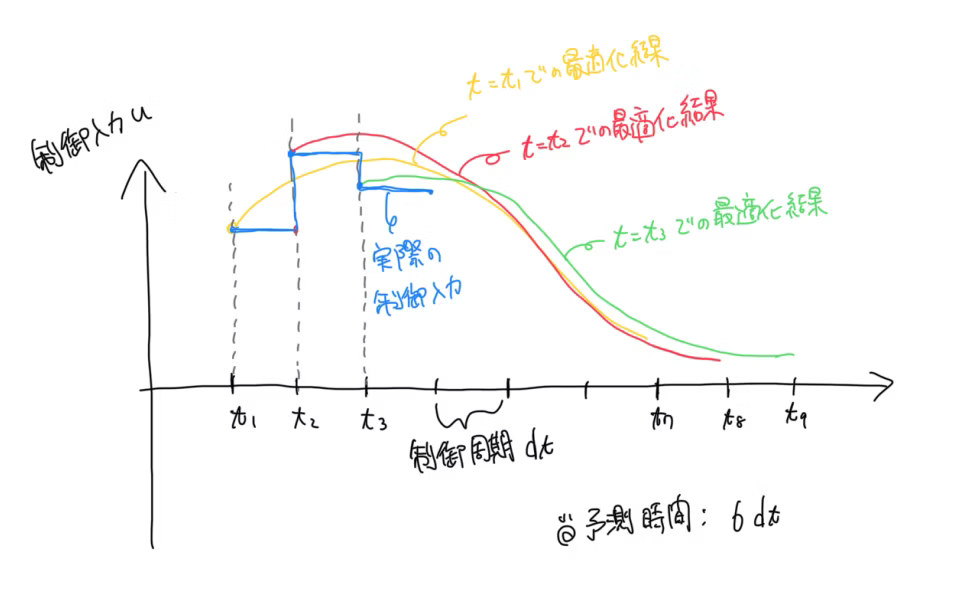
\includegraphics[clip, width = 10.0cm]{takahoribe.png}
        \end{figure}
        \centering
        \tiny{
            \rightline{
                \href{https://qiita.com/taka_horibe/items/47f86e02e2db83b0c570}{モデル予測制御(MPC)による軌道追従制御より}
            }
        }
        \footnotesize
        有限時間のLQRをシフトさせるイメージ
    \end{frame}

    \begin{frame}{MPC概略}
        \footnotesize

        \begin{block}{MPCで解く問題}
            \vspace{-1em}
            \begin{flalign*}
                & x_{k+1} = Ax_k+Bu_k \\
                & J =
                \tikz[remember picture, baseline=(T3.base)] {
                    \node [fill=orange!20!white, inner sep=0pt, outer sep=0, minimum height=4ex] (T3) {$\dfrac{1}{2} \left[ x_{N}^{T}Px_{N} \right]$};
                }
                +
                \tikz[remember picture, baseline=(T4.base)] {
                    \node [fill=red!20!white, inner sep=0pt, outer sep=0, minimum height=4ex] (T4) {$\dfrac{1}{2} \sum_{i=0}^{N-1} \left[x_{i}^TQx_{i} + u_{i}^TRu_{i} \right]$};
                }
            \end{flalign*}

            \begin{tikzpicture}[remember picture, overlay]
                \node [below=0pt of T3, text=orange!80!black] {終端コスト};
                \node [below=0pt of T4, text=red!80!black] {ステージコスト};
            \end{tikzpicture}
            \vspace{-1em}
        \end{block}
        \centering

        \vspace{-1em}
        \begin{align*}
            U = 
            \begin{bmatrix}
                u_0 & u_1 & \dots & u_{N-1}
            \end{bmatrix}^\top
        \end{align*}
        \vspace{-1em}

        \begin{enumerate}
            \item 
            \tikz[remember picture] \node[coordinate] (start) {};
            $J$が最小になるような$u_0^* \sim u_{N-1}^*$を求める
            \begin{enumerate}
                \item \colorbox{yellow}{既知変数$x_0$から未知変数$x_1 \sim x_N$を推定}
                \item $U$についての最適化問題に変形
                \item 最適化問題を解く
            \end{enumerate}
            \item 
            \tikz[remember picture] \node[coordinate] (end) {};
            $u_0^*$をシステムへの入力とする
        \end{enumerate}

        \begin{tikzpicture}[remember picture, overlay]
            \draw[->,thick] ([xshift=-0.6cm]end) -- ([xshift=-1.0cm]end) -- ([xshift=-1.0cm]start)-- ([xshift=-0.6cm]start);
        \end{tikzpicture}

    \end{frame}

    \begin{frame}{未知変数$x_1 \sim x_N$を推定($x_0$は現在の状態)}
        \footnotesize
        \fbox{\parbox{.9\textwidth}{
            行列形式:
            \[
                \begin{bmatrix}
                    x_1 \\
                    x_2 \\
                    \vdots \\
                    x_N
                \end{bmatrix}
                =
                \begin{bmatrix}
                    A \\
                    A^2 \\
                    \vdots \\
                    A^N
                \end{bmatrix}
                x_0
                +
                \begin{bmatrix}
                    B & 0 & \ldots & 0 \\
                    AB & B & \ldots & 0 \\
                    \vdots & \vdots & \ddots & \vdots \\
                    A^{N-1}B & A^{N-2}B & \ldots & B
                \end{bmatrix}
                \begin{bmatrix}
                    u_0 \\
                    u_1 \\
                    \vdots \\
                    u_{N-1}
                \end{bmatrix}
            \]
        }}
        \centering

        \begin{itemize}
            \item 1ステップ先の予測:
            \[
                x_1 = Ax_0 + Bu_0
            \]
            
            \item 2ステップ先の予測:
            \begin{align*}
                x_2 &= A(Ax_0 + Bu_0) + Bu_1 \\
                &= A^2x_0 + ABu_0 + Bu_1
            \end{align*}
            
            \item 一般的に \(N\) ステップ先の予測:
            \[
                x_N = A^Nx_0 + A^{N-1}Bu_0 + A^{N-2}Bu_1 + \ldots + Bu_{N-1}
            \]
            
        \end{itemize}
    \end{frame}

    \begin{frame}{MPC概略}
        \footnotesize
    
        \fbox{\parbox{.9\textwidth}{
            \begin{align*}
                J &= \dfrac{1}{2} \left[ x_{N}^{T}Px_{N} \right] + \dfrac{1}{2} \sum_{i=0}^{N-1} \left[x_{i}^TQx_{i} + u_{i}^TRu_{i} \right] \\
                \begin{bmatrix}
                    x_1 \\
                    x_2 \\
                    \vdots \\
                    x_N
                \end{bmatrix}
                &=
                \begin{bmatrix}
                    A \\
                    A^2 \\
                    \vdots \\
                    A^N
                \end{bmatrix}
                x_0
                +
                \begin{bmatrix}
                    B & 0 & \ldots & 0 \\
                    AB & B & \ldots & 0 \\
                    \vdots & \vdots & \ddots & \vdots \\
                    A^{N-1}B & A^{N-2}B & \ldots & B
                \end{bmatrix}
                \underbrace{
                    \begin{bmatrix}
                        u_0 \\
                        u_1 \\
                        \vdots \\
                        u_{N-1}
                    \end{bmatrix}
                }_{U}
            \end{align*}
        }}
        \centering
        
        \begin{enumerate}
            \item 
            \tikz[remember picture] \node[coordinate] (start) {};
            $J$が最小になるような$u_0^* \sim u_{N-1}^*$を求める
            \begin{enumerate}
                \item 既知変数$x_0$から未知変数$x_1 \sim x_N$を推定
                \item \colorbox{yellow}{$U$についての最適化問題に変形}
                \item 最適化問題を解く
            \end{enumerate}
            \item 
            \tikz[remember picture] \node[coordinate] (end) {};
            $u_0^*$をシステムへの入力とする
        \end{enumerate}

        \begin{tikzpicture}[remember picture, overlay]
            \draw[->,thick] ([xshift=-0.6cm]end) -- ([xshift=-1.0cm]end) -- ([xshift=-1.0cm]start)-- ([xshift=-0.6cm]start);
        \end{tikzpicture}
    
    \end{frame}

    \begin{frame}{$U$についての最適化問題に変形1}
        \footnotesize

        \begin{block}{二次計画問題への変形}
            \begin{align*}
                J &= \dfrac{1}{2} \left[ x_{N}^{T}Px_{N} \right] + \dfrac{1}{2} \sum_{i=0}^{N-1} \left[x_{i}^TQx_{i} + u_{i}^TRu_{i} \right] \\
                &= \colorbox{yellow}{$\frac{1}{2} U^T H U + g(x_0)^T U$} + c(x_0)
            \end{align*}
            \centerline{
                {
                    \color{red} $c(x_0)$は$U$が含まれていないので無視できる
                }
            }
        \end{block}

        評価関数が二次になっていることを利用する \\
        二次の最適化関数を持つ問題は、一般に二次計画問題(QP)として知られる
        \begin{align*}
            \min _x \frac{1}{2} x^T Q x + c^T x \qquad
            s.t & Ax \leq b \\
             & Gx = h
        \end{align*}
    \end{frame}
    
    \begin{frame}{$U$についての最適化問題に変形2}
        \tiny

        \begin{align*}
            U &= 
            \begin{bmatrix}
                u(0) \\
                u(1) \\
                \vdots \\
                u(N-1)
            \end{bmatrix}, &
            \mathcal{A} &= 
            \begin{bmatrix}
                A \\
                A^2 \\
                \vdots \\
                A^N
            \end{bmatrix}, &
            \mathcal{B} &=
            \begin{bmatrix}
                B & 0 & \ldots & 0 \\
                AB & B & \ldots & 0 \\
                \vdots & \vdots & \ddots & \vdots \\
                A^{N-1}B & A^{N-2}B & \ldots & B
            \end{bmatrix} \\
            H &= \left(\mathcal{B}^T \mathcal{Q B} + \mathcal{R}\right), &
            g(x_0) &= \mathcal{B}^T \mathcal{Q} \mathcal{A} x_0, &
            c(x_0) &= \frac{1}{2} x_0^T\left(\mathcal{A}^T \mathcal{Q} \mathcal{A} + Q\right) x_0 \\
            \mathcal{Q} &= \left[\begin{array}{cccc}
            Q & & & \\
            & \ddots & & \\
            & & Q & \\
            & & & P
            \end{array}\right], &
            \mathcal{R} &= \left[\begin{array}{ccc}
            R & & \\
            & \ddots & \\
            & & R
            \end{array}\right]
        \end{align*}
    \end{frame}


    \begin{frame}{MPC概略}
        \footnotesize
    
        \fbox{\parbox{.9\textwidth}{
            \begin{align*}
                J &= \frac{1}{2} U^T H U + g(x_0)^T U + c(x_0) \\
                U^* &= \min _U J
            \end{align*}
        }}
        \centering
        
        \begin{enumerate}
            \item 
            \tikz[remember picture] \node[coordinate] (start) {};
            $J$が最小になるような$u_0^* \sim u_{N-1}^*$を求める
            \begin{enumerate}
                \item 既知変数$x_0$から未知変数$x_1 \sim x_N$を推定
                \item $U$についての最適化問題に変形
                \item \colorbox{yellow}{最適化問題を解く}
            \end{enumerate}
            \item 
            \tikz[remember picture] \node[coordinate] (end) {};
            $u_0^*$をシステムへの入力とする
        \end{enumerate}
        
        \begin{tikzpicture}[remember picture, overlay]
            \draw[->,thick] ([xshift=-0.6cm]end) -- ([xshift=-1.0cm]end) -- ([xshift=-1.0cm]start)-- ([xshift=-0.6cm]start);
        \end{tikzpicture}
    
    \end{frame}

    \begin{frame}{二次計画問題(QP)}
        \footnotesize
        
        \vspace{-1.5em}
        \begin{align*}
            \min _x \frac{1}{2} x^T Q x + c^T x \qquad
            s.t \quad & Ax \leq b \\
             & Gx = h
        \end{align*}

        \begin{block}{KKT条件}
            \vspace{-1em}
            \begin{align*}
                Qx + c - A^T \lambda - G^T \mu &= 0 \\
                Ax - b &= 0 \\
                Gx - h &= 0 \\
                \mu &\geq 0 \\
                \mu_i (Gx - h)_i &= 0 \quad \text{for } i = 1,2,\ldots,m
            \end{align*}
            \vspace{-3em} 
            \begin{itemize}
                \item \( \lambda \): 等式制約のLagrange乗数ベクトル
                \item \( \mu \): 不等式制約のLagrange乗数ベクトル
            \end{itemize}
        \end{block}
        
        \centerline{
            \color{red}{KKT条件を満たす解を見つければいい!!!}
        }
    \end{frame}           

    \begin{frame}{MPC(線形)で重要なのは二次計画法}
        \footnotesize

        \begin{tcolorbox}[title=数値計算を用いてKKT条件を満たす解を求める]
            \tikz[remember picture] \node[coordinate] (newton) {};
            {Newton法}   
            \qquad \colorbox{yellow}{制約条件が無いor等式制約のみ}の凸最適化 \\
            \par
            \tikz[remember picture] \node[coordinate] (active_set) {};
            {有効制約法}
            \quad \; \colorbox{yellow}{比較的小規模〜中規模}の凸最適化 \\
            \par
            \tikz[remember picture] \node[coordinate] (interior) {};
            {内点法}
            \qquad \quad \; \colorbox{yellow}{大規模}な凸最適化 \\
            
            \begin{tikzpicture}[remember picture, overlay]
                \draw[thick] ([xshift=0.1cm]newton) -- ([xshift=-0.2cm]newton) -- ([xshift=-0.2cm]active_set) -- ([xshift=-0.2cm]interior) -- ([xshift=0.1cm]interior);
                \draw[thick] ([xshift=0.1cm]active_set) -- ([xshift=-0.2cm]active_set);
            \end{tikzpicture}
            \vspace{-2.5em}
        \end{tcolorbox}
        凸関数で制約が凸集合
        \tikz \draw [arrows = {-Stealth[inset=0pt, length=5pt, angle'=30]}](0,0) -- (0.5,0);
        \colorbox{yellow}{最適化問題の解が大域的最適解} \\
        {\small \textbf{\color{red}{どの手法で二次計画問題を解くのかでMPCの性能が決まる!!!}}}
    \end{frame}

    \begin{frame}{Newton法1}
        \footnotesize

        \fbox{\parbox{.9\textwidth}{
            \begin{align*}
                \min _x f(x) \qquad \text{s.t.} \quad g(x) = 0
            \end{align*}
        }}
        \centering
        \begin{flushleft}
            Lagrange関数を$L(x) = f(x) + \lambda^T  g(x)$と定義すると, \\
            最適解の必要条件は次式となる
        \end{flushleft}
        \begin{equation*}
            \nabla L\left(x\right) = 0
        \end{equation*}
        \leftline{
            最適解の十分条件はヘッセ行列$\nabla ^2 f\left(x\right)$が正定値
        }

        \begin{tcolorbox}[title=Newton法のPoint]
            $\nabla L\left(x\right) = 0$の連立方程式を解くのは困難
            
            \tikz \draw [arrows = {-Stealth[inset=0pt, length=5pt, angle'=30]}]
            (0,0) -- (0,-0.5);
        
            更新式$x_{k+1}=x_k+d$を用いて$\nabla L\left(x\right)=0$を解く
        \end{tcolorbox}
    \end{frame}  
    
    \begin{frame}{Newton法2}
        \footnotesize

        \fbox{\parbox{.9\textwidth}{
            \centering
            $\nabla L \left(x\right)=0$ \qquad
            更新式:$x_{k+1}=x_k+\colorbox{yellow}{$d$}$
        }}
        \vspace{1em}

        \begin{itemize}
            \item $\nabla L \left (x_k+d \right )$をTaylor展開をする
            \begin{equation*}
                \nabla L\left(x_k + d\right) \simeq \nabla L\left(x_k\right)+\nabla ^ 2 L\left(x_k\right)d
            \end{equation*}
            \item $\nabla L \left(x\right)=0$では$\nabla L \left(x_k + d\right)$が0になる
            \begin{equation*}
                \nabla L\left(x_k\right)+\nabla ^ 2 L\left(x_k\right)d=0 \iff \colorbox{yellow}{$d =-\nabla ^2 L\left(x_k\right) ^ {-1} \nabla L \left(x_k\right)$}
            \end{equation*}
        \end{itemize}

        \begin{block}{Newton法}
            \begin{enumerate}
                \item 初期点$x_0$を定め、$k=0$とする
                \item $\lVert \nabla L\left(x_k\right) \rVert$が十分に小さければ終了
                \item $x_{k+1}=x_k-\nabla ^2 L\left(x_k\right) ^ {-1} \nabla L \left(x_k\right)$
            \end{enumerate}
        \end{block}

    \end{frame}

    \begin{frame}{内点法}
        \footnotesize
        \centering

        \begin{itemize}
            \item 不等式制約を持つ凸最適化問題を解ける
            \item 主双対内点法は主内点法よりも高速
            \item ベースはニュートン法
        \end{itemize}
        \begin{tikzpicture}
            % ノードの定義
            \node (interior_graph) {内点法};
            \node (primal_interior_graph) [above right=0.1cm and 2cm of interior_graph] {主内点法};
            \node (primal_dual_interior_graph) [below right=0.1cm and 2cm of interior_graph] {主双対内点法};
        
            % 線の引き方
            \draw (interior_graph.east) -- ++(1cm,0) |- (primal_interior_graph.west);
            \draw (interior_graph.east) -- ++(1cm,0) |- (primal_dual_interior_graph.west);
        \end{tikzpicture}
    \end{frame}

    \begin{frame}{主内点法1}
        \footnotesize

        \begin{tcolorbox}[title=主内点法のPoint]
            不等式制約があると最適化が難しくなる \\
            \vspace{-2em}
            \begin{align*}
                \min _x f\left(x\right) \qquad
                s.t \quad & g\left(x\right) = 0 \\
                 & x \geq 0
            \end{align*}
            \centerline{
                \tikz \draw [arrows = {-Stealth[inset=0pt, length=5pt, angle'=30]}]
                (0,0) -- (0,-0.5); \\
            }

            \colorbox{yellow}{バリア関数}によって不等式制約を最小化する関数に含める
            \begin{flalign*}
                \min _x f(x)
                \tikz[remember picture, baseline=(T3.base)] {
                    \node [fill=yellow, inner sep=0pt, outer sep=0, minimum height=4ex] (T3) {$-\nu \sum_{i=1}^l \log \left(x_i\right)$};
                } \qquad
                s.t \quad g\left(x\right) = 0
            \end{flalign*}
        \end{tcolorbox}
        \centerline{
            {\small \textbf{等式制約のみになったのでNewton法で解ける!!!}}
        }
    \end{frame}

    \begin{frame}{主内点法2}
        \footnotesize
        \begin{figure}[H]
            \centering
            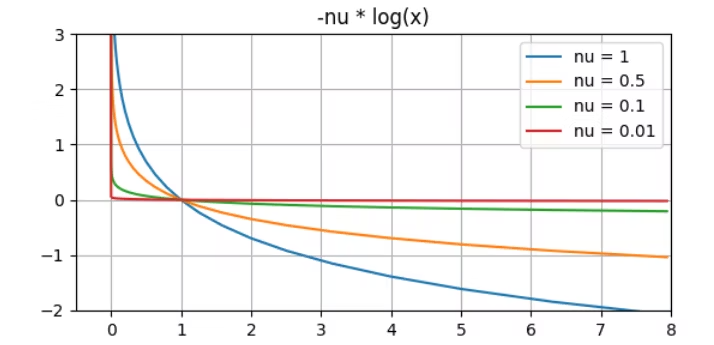
\includegraphics[clip, width = 10.0cm]{barrier.png}
        \end{figure}
        \centering
        \tiny{
            \rightline{
                \href{https://qiita.com/taka_horibe/items/47f86e02e2db83b0c570}{モデル予測制御(MPC)による軌道追従制御より}
            }
        }
        \footnotesize
        \begin{itemize}
            \item 初期点として実行可能な点を与える必要がある
            \item 制約の境界付近ではNewton法の数値計算が解けない場合もある
        \end{itemize}
    \end{frame}

    \begin{frame}{主双対内点法1}
        \footnotesize

        \fbox{\parbox{.9\textwidth}{
            \begin{align*}
                \min _x \frac{1}{2} {x}^T {Qx} + {c}^T {x} \qquad
                \text{ s.t. } {Ax} = {b}, \, {x} \geq 0
            \end{align*}
        }}
        \centering
        
        \begin{align*}
            &{Ax} = {b}, && {x} \geq 0 \\
            &{A}^T {\lambda} + \mu = {Qx} + {c}, && \mu \geq 0 \\
            &{x}^T \mu = 0
        \end{align*}
                    
        \begin{tcolorbox}[title={$x$, $\lambda$, $\mu$全てに対してニュートン法を行う}]
            \vspace{-1em}
            \begin{align*}
                &x_{k+1} = x_k + dx \\
                &\lambda_{k+1} = \lambda_k + d\lambda \\
                &\mu_{k+1} = \mu_k + d\mu
            \end{align*}
        \end{tcolorbox}
        

    \end{frame}
    
    \begin{frame}{主双対内点法2}
        \footnotesize
        \vspace{-2em}
        \begin{align*}
            &{Ax} = {b}\\
            &{A}^T {\lambda} + \mu = {Qx} + {c}\\
            &{x}^T \mu = 0
        \end{align*}
        \vspace{-2em}
        \begin{itemize}
            \item Newton法と同様に扱う変数($x$,$\lambda$,$\mu$)を一次近似する($dXd\mu=0$)
        \end{itemize}
        \vspace{-1.5em}
        \begin{align*}
            &A(x_k + dx) = b \\
            &A^T (\lambda + d\lambda) + (\mu_k + d\mu) = Q(x_k + dx) + c \\
            &X_k\mu_k + X_kd\mu + \mu_kdX = \colorbox{yellow}{$0$}
        \end{align*}

        \begin{itemize}
            \item 通常のNewton法はここで$dx$,$d\lambda$, $d\mu$についてまとめる
            \item 主双対内点法はここで中心パスを導入し、これに沿った解を得ることで最適解に近づく
        \end{itemize}
        \begin{align*}
            X_k\mu_k + X_kd\mu + \mu_kdX &= \colorbox{yellow}{$\sigma \nu _k$} = \colorbox{yellow}{$\sigma \frac{1}{N} \sum_{i} (x_i \mu_i)^k$}
        \end{align*}
      
    \end{frame}

    \begin{frame}{主双対内点法3}
        \footnotesize
        \begin{block}{主双対内点法}
            \begin{align*}
                \begin{bmatrix}
                A & 0 & 0 \\
                -Q & A^T & I \\
                M_k & 0 & X_k
                \end{bmatrix}
                \begin{bmatrix}
                d x \\
                d \lambda \\
                d \mu
                \end{bmatrix}
                &=
                \begin{bmatrix}
                b - Ax_k \\
                Qx_k + c - A^T \lambda_k - \mu_k \\
                \sigma \nu_k e - X_k \mu_k
                \end{bmatrix},
                \end{align*}
                \begin{align*}
                X_k &= \text{diag}(x_{k1}, \dots, x_{kn}), \\
                M_k &= \text{diag}(\mu_{k1}, \dots, \mu_{kl}), \\
                e &= [1, \dots, 1]^T.
            \end{align*}
        \end{block}
        \begin{itemize}
            \item Newton法と同様、更新式として解く
            \item 初期値として実行可能な点(内点)を与える必要がある
        \end{itemize}
    \end{frame}
    \begin{frame}{MPC概略}
        \footnotesize
    
        \fbox{\parbox{.9\textwidth}{
            \begin{align*}
                J &= \frac{1}{2} U^T H U + g(x_0)^T U + c(x_0) \\
                U^* &= 
                \begin{bmatrix}
                    u^*(0) \\
                    u^*(1) \\
                    \vdots \\
                    u^*(N-1)
                \end{bmatrix} = \min _U J
            \end{align*}
        }}
        \centering
        
        \begin{enumerate}
            \item 
            \tikz[remember picture] \node[coordinate] (start) {};
            $J$が最小になるような$u_0^* \sim u_{N-1}^*$を求める
            \begin{enumerate}
                \item 既知変数$x_0$から未知変数$x_1 \sim x_N$を推定
                \item $U$についての最適化問題に変形
                \item 最適化問題を解く
            \end{enumerate}
            \item 
            \tikz[remember picture] \node[coordinate] (end) {};
            \colorbox{yellow}{$u_0^*$をシステムへの入力とする}
        \end{enumerate}
        
        \begin{tikzpicture}[remember picture, overlay]
            \draw[->,thick] ([xshift=-0.6cm]end) -- ([xshift=-1.0cm]end) -- ([xshift=-1.0cm]start)-- ([xshift=-0.6cm]start);
        \end{tikzpicture}
    \end{frame}

    \begin{frame}{MPCのイメージ}
        \footnotesize

        \begin{figure}[H]
            \centering
            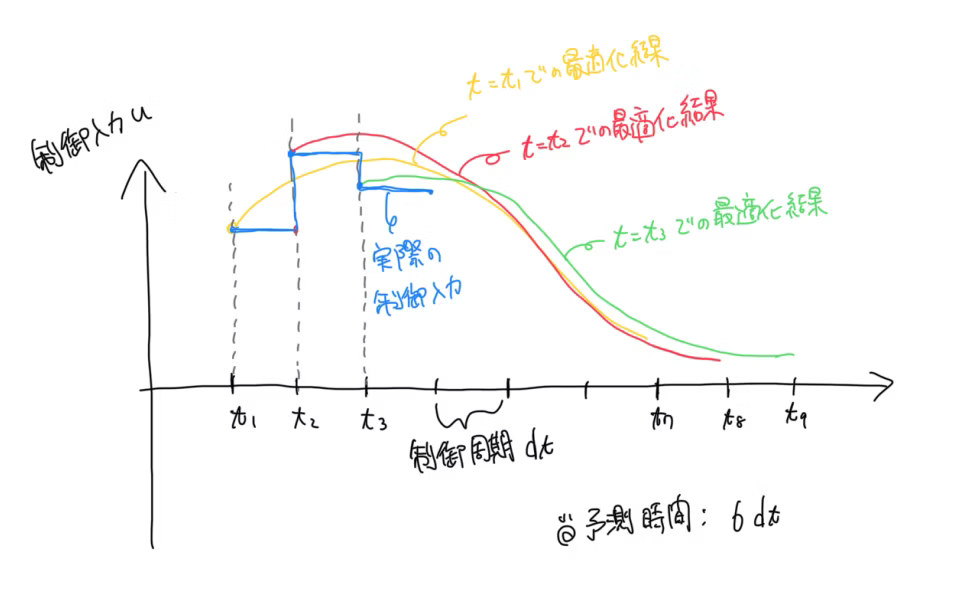
\includegraphics[clip, width = 10.0cm]{takahoribe.png}
        \end{figure}
        \centering
        \tiny{
            \rightline{
                \href{https://qiita.com/taka_horibe/items/47f86e02e2db83b0c570}{モデル予測制御(MPC)による軌道追従制御より}
            }
        }
    \end{frame}

    \begin{frame}{参考資料}
        \footnotesize

        書籍\\
        \begin{itemize}
            \item しっかり学ぶ数理最適化
        \end{itemize}

        サイト(URL) \\
        \begin{itemize}
            \item MyEnigmaのMPC導入: \href{https://myenigma.hatenablog.com/entry/2016/07/25/214014}{https://myenigma.hatenablog.com/entry/2016/07/25/214014}
            \item MyEnigmaのMPC数式: \href{https://myenigma.hatenablog.com/entry/2017/02/07/084922}{https://myenigma.hatenablog.com/entry/2017/02/07/084922}
            \item MPCの具体例: \href{https://ramune6110.hatenablog.com/entry/2022/02/13/154405}{https://ramune6110.hatenablog.com/entry/2022/02/13/154405}
            \item MPCを用いた倒立振子: \href{https://qiita.com/slowsingle/items/f3074ea6670da42696e0}{https://qiita.com/slowsingle/items/f3074ea6670da42696e0}
            \item MPCの説明と実機を用いた実験: \href{http://www.kostasalexis.com/linear-model-predictive-control.html}{http://www.kostasalexis.com/linear-model-predictive-control.html}
        \end{itemize}
    \end{frame}
    
\end{document}